\documentclass{classrep}
\usepackage[utf8]{inputenc}
\usepackage{amsmath}
\usepackage{graphicx}
\usepackage{url}
\usepackage{hyperref}
\usepackage[T1]{fontenc}
\usepackage[polish]{babel}
\usepackage[utf8]{inputenc}
\usepackage{lmodern}
\usepackage{color}
\selectlanguage{polish}
\graphicspath{ {./rys/} }



\studycycle{Informatyka, studia dzienne, inż I st.}
\coursesemester{VI}

\coursename{Sztuczna inteligencja i systemy ekspertowe}
\courseyear{2019/2020}

\courseteacher{dr inż. Krzysztof Lichy}
\coursegroup{wtorek, 10:30}

\author{
  \studentinfo{Radosław Grela}{216769} \and
  \studentinfo{Jakub Wąchała}{216914}
}

\title{Zadanie 1: Piętnastka}

\begin{document}
\maketitle

\newpage

\section{Cel} % 1. Cel %
W tym zadaniu należało napisać program, który będzie rozwiązywał układankę pod nazwą \textsl{Piętnastka (Fifteen Puzzle)}.
Następnie, należało przebadać układy początkowe układanki w odległościach 1-7 od układu wzorcowego (413 układów)
korzystając z różnych strategii i przypadków przeszukiwania sąsiedztwa.

\section{Wprowadzenie} % 2. Wprowadzenie %
\textsl{Piętnastka}, potocznie też \textsl{Przesuwanka} to prosta gra logiczna, w której zadaniem jest ułożyć 15 ponumerowanych kwadratowych klocków umieszczonych w pudełku 4x4. Pozostałe, 16 miejsce jest puste, co pozwala na poruszanie elementów układanki.\cite{pierwszymath} 
\begin{figure}[h!]
    \centering
    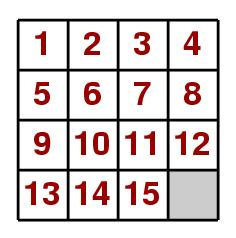
\includegraphics[width=0.25\textwidth]{15grid1.jpg}
    \caption{Ułożona piętnastka. \cite{pierwszymath}}
\end{figure}

W programie przez nas napisanym mamy do wyboru 3 strategie przestrzeni stanów:
\begin{itemize}
\item Strategia wszerz BFS (\textsl{breadth-first search})
\item Strategia w głąb DFS (\textsl{depth-first search})
\item Strategia najpierw najlepszy A* z heurystykami Hamminga i Manhattan.
\end{itemize}
Strategie te są przykładem przeszukiwania drzewa. Jego węzłami są stany, czyli aktualne ułożenia układanki.
W części badawczej badaliśmy tylko układanki rozmiarów 4x4, jednak nasz program dopuszcza także niestandardowe rozmiary.

\subsection{DFS} % 2.1 DFS %
Badanie grafu strategią DFS polega na przejściu wszystkich krawędzi wychodzących z podanego wierzchołka. Jest to algorytm rekurencyjny. Kolejność przechodzenia po drzewie przedstawiona jest na rysunku (\ref{kolejnoscDFS}).
 \begin{figure}[h!]
    \centering
    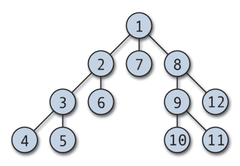
\includegraphics[width=0.5\textwidth]{dfs.png}
    \caption{Kolejność przechodzenia w algorytmie DFS. \cite{wikiDFS}}
    \label{kolejnoscDFS}
\end{figure}
Gdy rozwiązanie zostanie znalezione, wystarczy wrócić rekurencyjnie do rodzica.

\subsection{BFS} % 2.2 BFS %
Algorytm BFS polega na przejściu przez wszystkich sąsiadów danego wierzchołka. Następnie, należy kontynuować czynność dalej, dopóki nie odwiedzimy wszystkich sąsiadów sąsiadów. Kolejność przechodzenia po drzewie jest pokazana na rysunku (\ref{kolejnoscBFS}).
\begin{figure}[h!]
    \centering
    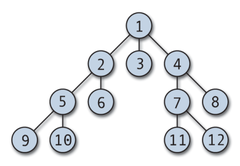
\includegraphics[width=0.5\textwidth]{bfs.png}
    \caption{Kolejność przechodzenia w algorytmie BFS. \cite{wikiBFS}}
    \label{kolejnoscBFS}
\end{figure}

\subsection{A*} % 2.3 A* %
A* to kolejna strategia przeszukiwania grafu. Bazuje ona na funkcji 
\begin{equation}
	f(x) = g(x) + h(x) 
	\label{fun}
\end{equation}
gdzie $g(x)$ oznacza głębokość, a $h(x)$ to wartość odpowiedniej funkcji miary błędu. W naszym programie wykorzystujemy następujące dwie metryki:

\subsubsection{Metryka Hamminga} % 2.3.1 Hamming %
W metryce Hamminga jako wynik funkcji $h(x)$ użytej we wzorze (\ref{fun}) podawana jest ilość klocków, która nie znajduje się na swojej pozycji. Przykładowo dla układanki na rysunku (\ref{blednaukladanka}) wynik takiej funkcji będzie równy 5 (elementy 0, 3, 4, 8 i 12 nie znajdują się na swoich pozycjach).
\begin{figure}[h!]
    \centering
    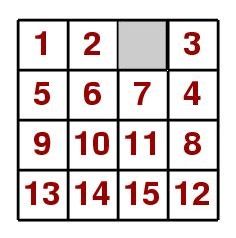
\includegraphics[width=0.25\textwidth]{15wrong1.jpg}
    \caption{Przykładowa błędnie ułożona układanka.}
	\label{blednaukladanka}
\end{figure}

\subsubsection{Metryka Manhattan}  % 2.3.2 Manhattan %
W tej metryce wynikiem funkcji $h(x)$ użytej we wzorze (\ref{fun}) jest suma wartości bezwzględnych różnic współrzędnych między punktem, w którym klocek powinien się znaleźć, a punktem, w którym jest obecnie. Dla rysunku (\ref{blednaukladanka}) wynik to 8 (4 + 1 + 1 + 1 + 1).

\section{Opis implementacji} % 3. Opis implementacji %
Napisany przez nas program jest aplikacją konsolową napisaną w języku Java. Jako parametry programu należy podać 5 argumentów:
\begin{enumerate}
\item strategia (dfs, bfs, astr)
\item porządek (jeżeli jest to strategia DFS lub BFS) lub heurystyka (dla metody A*). 
\item ścieżka do pliku z zadaną układanką do ułożenia
\item ścieżka do pliku, w którym zostanie zapisane rozwiązanie
\item ścieżka do pliku, w którym zostaną zapisane dodatkowe informacje dot. przeprowadzonego procesu
\end{enumerate}
Poniżej przedstawiamy krótki opis, jak zostały zaimplementowane poszczególne strategie.

\subsection{DFS} % 3.1 DFS %
Do przechowywania stanów nie używamy specjalnej struktury danych, lecz za pomocą rekurencji program wie, który węzęł musi odwiedzić jako następny. Zatem przechowywanie stanów jest możliwe dzięki odkładaniu wywołań funkcji na stosie.

\subsection{BFS} % 3.2 BFS %
Dla algorytmu BFS wykorzystywane są dwie \textsl{ArrayListy}, które przechowują stany. Jedna z nich przechowuje węzły do odwiedzenia, a druga węzły odwiedzone. Spełniają one funkcję kolejki - nowe elementy dodawane są na koniec listy, a niepotrzebne już elementy znajdujące się na początku listy są usuwane.

\subsection{A*} % 3.3 A* %
W przypadku algorytmów A* dane są przetrzymywane na liście (ArrayList), która spełnia zadania kolejki priorytetowej. W momencie dodania nowego elementu na liście, jest ona sortowana zgodnie z wynikiem funkcji (\ref{fun}). Na początku listy znajdują się ''najgorsze'' elementy - te, których wartość funkcji jest największa, a na końcu elementy, które mają wartość tej funkcji najmniejszą.

Na poniższym rysunku przedstawiony jest uproszczony diagram UML naszego programu.
\begin{figure}[h!]
    \centering
    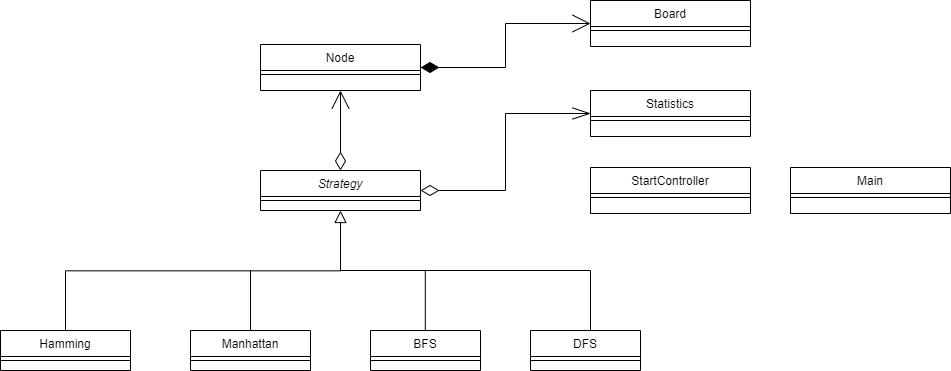
\includegraphics[width=1.2\textwidth]{uml.png}
    \caption{Diagram UML.}
\end{figure}
\newpage

\section{Materiały i metody} % 4. Materiały i metody %
Do przeprowadzenia badań nad utworzoną przez nas aplikacją użyliśmy kilku programów znajdujących się na stronie przedmiotu na Wikampie.
\begin{enumerate}
\item Program do utworzenia 413 różnych układów piętnastki z głębokością 1-7
\item Skrypt uruchamiający naszą aplikację z każdym algorytmem oraz ewentualną heurystyką i kolejnością
\item Skrypt Podsumowujący uzyskane wyniki z poprzedniego skryptu
\end{enumerate}
Otrzymane wyniki przedstawiliśmy na wykresach w następnej sekcji.

\section{Wyniki} % 5. Wyniki %
Na poniższych wykresach przedstawiliśmy średnie wartości:
\begin{itemize}
\item Czasu wykonywania
\item Maksymalnej głębokości
\item Ilości przetworzonych węzłów
\item Ilości odwiedzonych węzłów
\item Długości rozwiązania
\end{itemize}
Każdy wykres został wykonany dla każdej strategii oraz ich heurystyk.

\newpage
\subsection{Czas wykonania}
%%%% czas wykonania %%%%
\begin{figure}[h!]
    \centering
    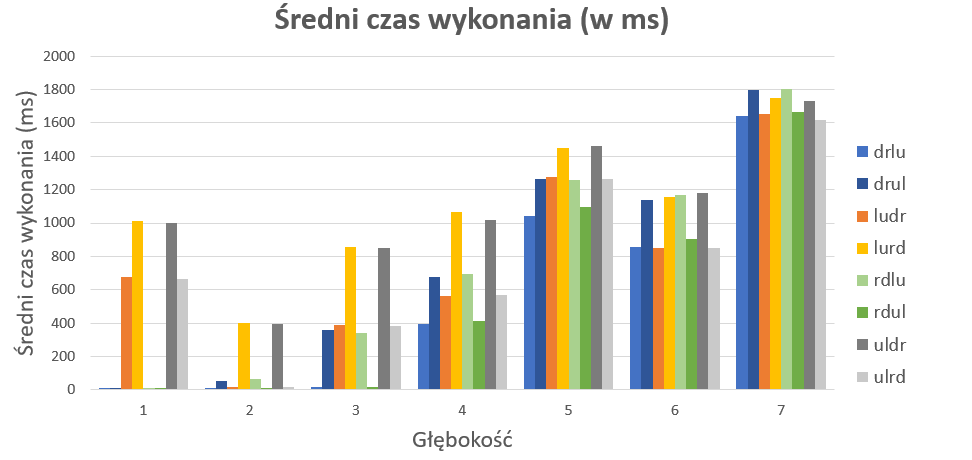
\includegraphics[width=0.83\textwidth]{czasdfs.png}
    \caption{Średni czas wykonania dla algorytmu DFS}
	\label{czasDFS}
\end{figure}
\begin{figure}[h!]
    \centering
    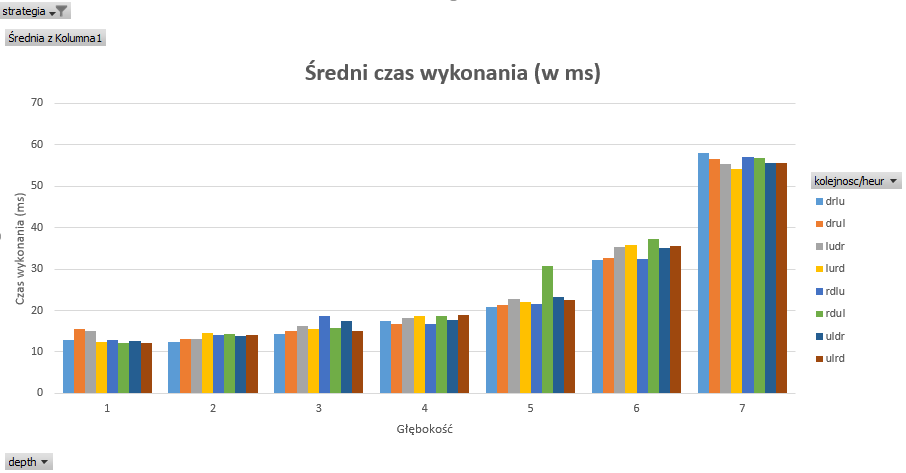
\includegraphics[width=0.85\textwidth]{czasbfs.png}
    \caption{Średni czas wykonania dla algorytmu BFS}
	\label{czasBFS}
\end{figure}
\begin{figure}[h!]
    \centering
    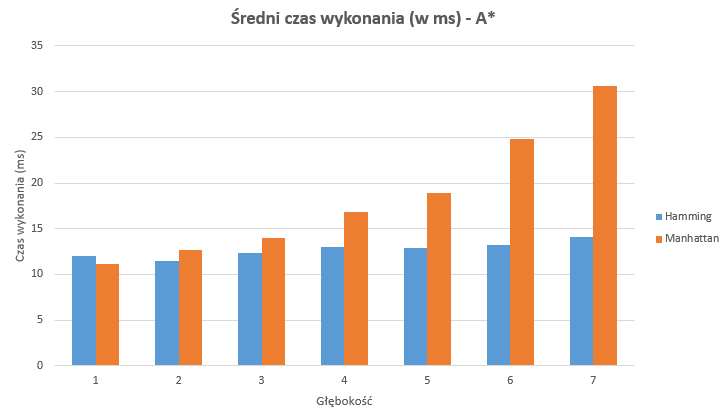
\includegraphics[width=0.85\textwidth]{czasastr.png}
    \caption{Średni czas wykonania dla algorytmu A*}
	\label{czasASTR}
\end{figure}

\newpage
\subsection{Maksymalna głębokość}
%%%% max depth %%%%
\begin{figure}[h!]
    \centering
    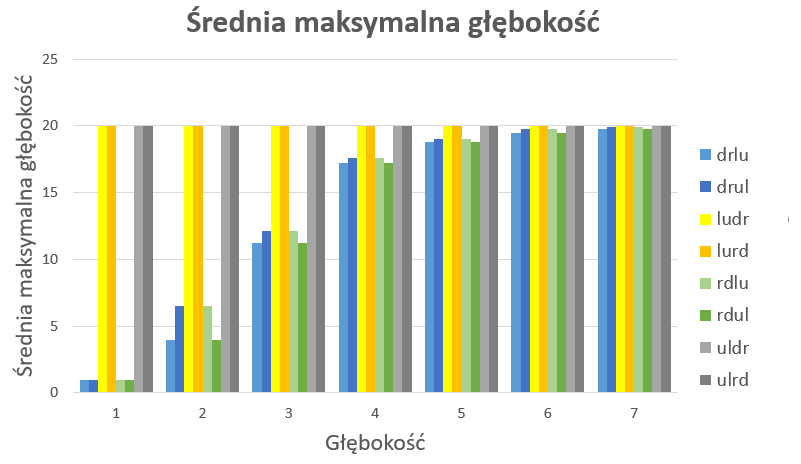
\includegraphics[width=0.89\textwidth]{maxdepthDFS.png}
    \caption{Średnia maksymalna głębokość dla algorytmu DFS}
	\label{maxdepthDFS}
\end{figure}
\begin{figure}[h!]
    \centering
    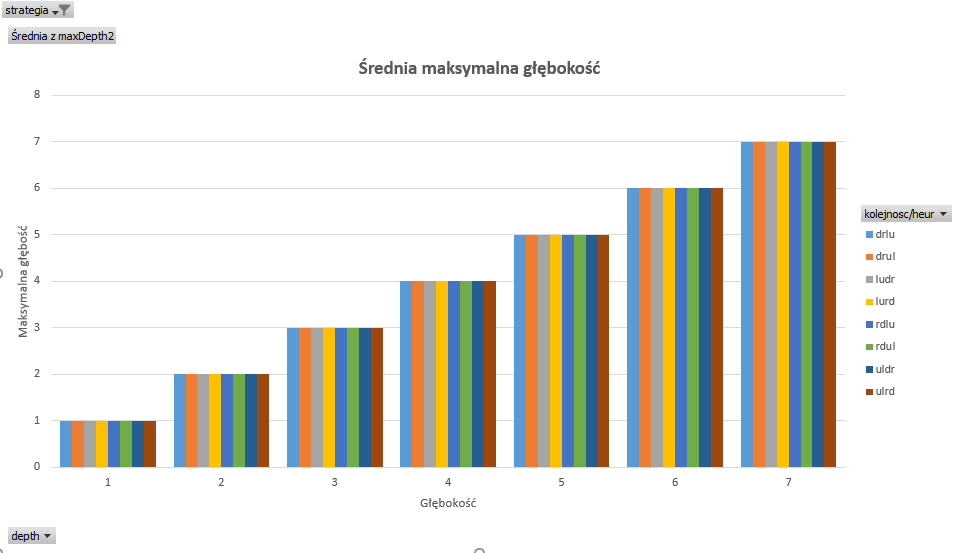
\includegraphics[width=0.83\textwidth]{maxdepthBFS.png}
    \caption{Średnia maksymalna głębokość dla algorytmu BFS}
	\label{maxdepthBFS}
\end{figure}
\begin{figure}[h!]
    \centering
    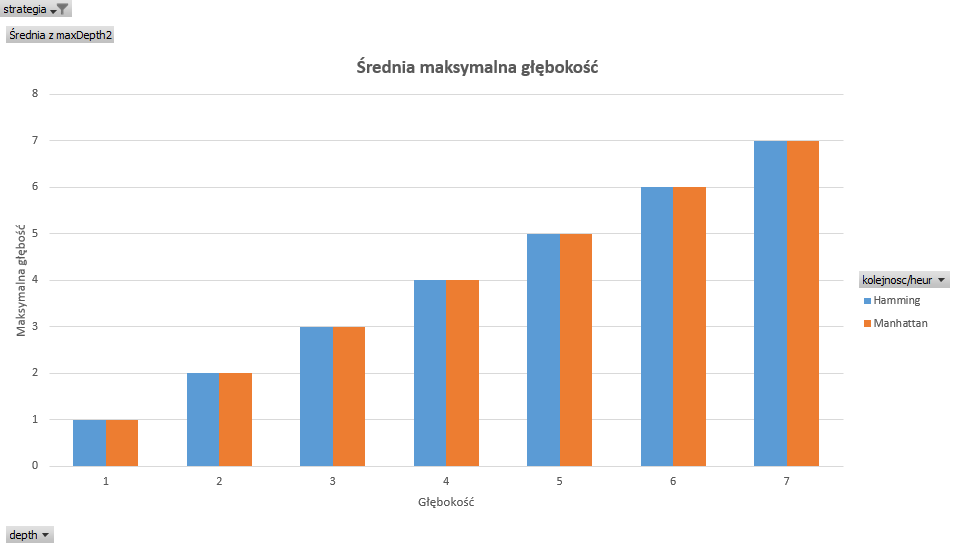
\includegraphics[width=0.83\textwidth]{maxdepthAstar.png}
    \caption{Średnia maksymalna głębokość dla algorytmu A*}
	\label{maxdepthASTR}
\end{figure}

\newpage
\subsection{Ilość przetworzonych węzłów}
%%%% przetworzone węzły %%%%
\begin{figure}[h!]
    \centering
    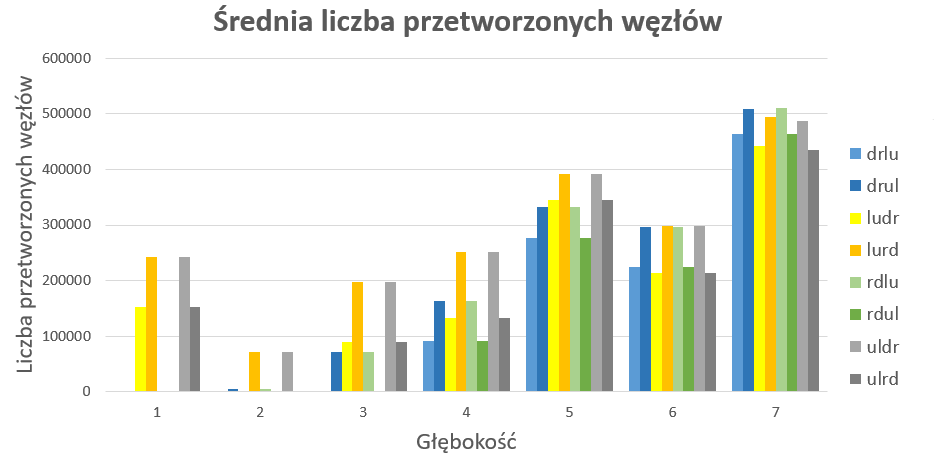
\includegraphics[width=0.83\textwidth]{processedDFS.png}
    \caption{Średnia ilość przetworzonych węzłów dla algorytmu DFS}
	\label{processedDFS}
\end{figure}
\begin{figure}[h!]
    \centering
    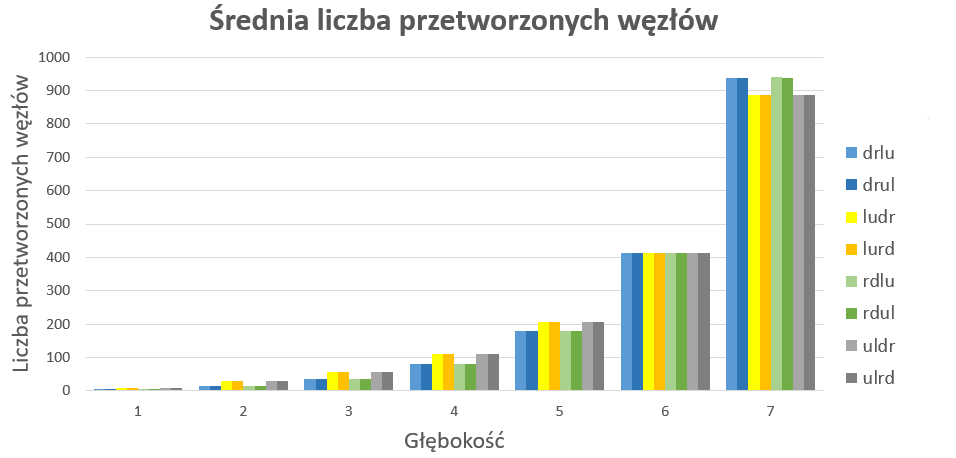
\includegraphics[width=0.83\textwidth]{processedBFS.png}
    \caption{Średnia ilość przetworzonych węzłów dla algorytmu BFS}
	\label{processedBFS}
\end{figure}
\begin{figure}[h!]
    \centering
    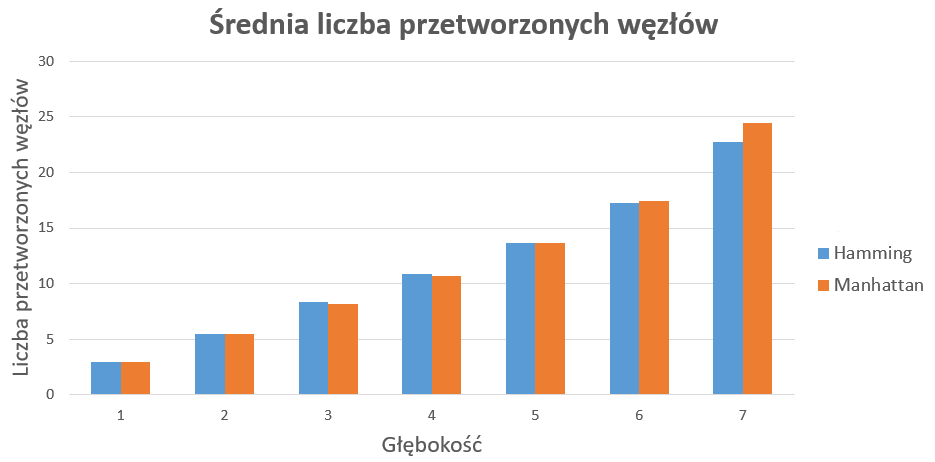
\includegraphics[width=0.83\textwidth]{processedastar.png}
    \caption{Średnia ilość przetworzonych węzłów dla algorytmu A*}
	\label{processedASTR}
\end{figure}

\newpage
\subsection{Ilość odwiedzonych węzłów}
%%%% odwiedzone węzły %%%%
\begin{figure}[h!]
    \centering
    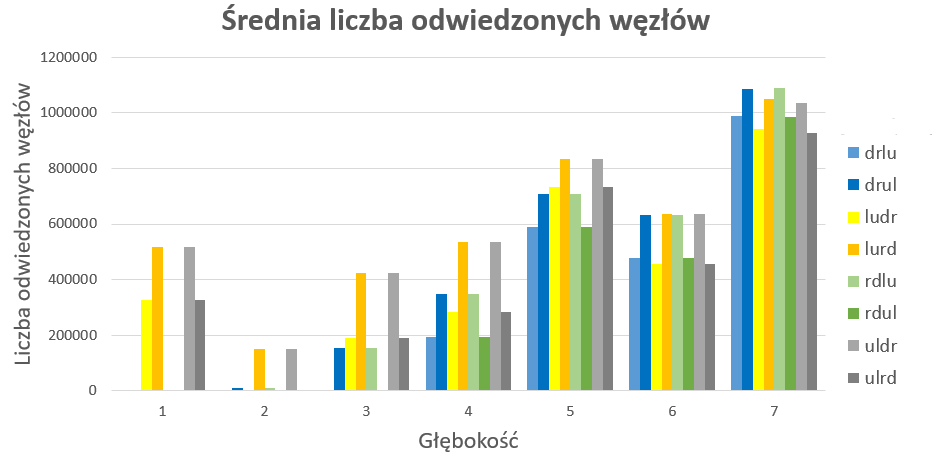
\includegraphics[width=0.83\textwidth]{visitedDFS.png}
    \caption{Średnia ilość odwiedzonych węzłów dla algorytmu DFS}
	\label{visitedDFS}
\end{figure}
\begin{figure}[h!]
    \centering
    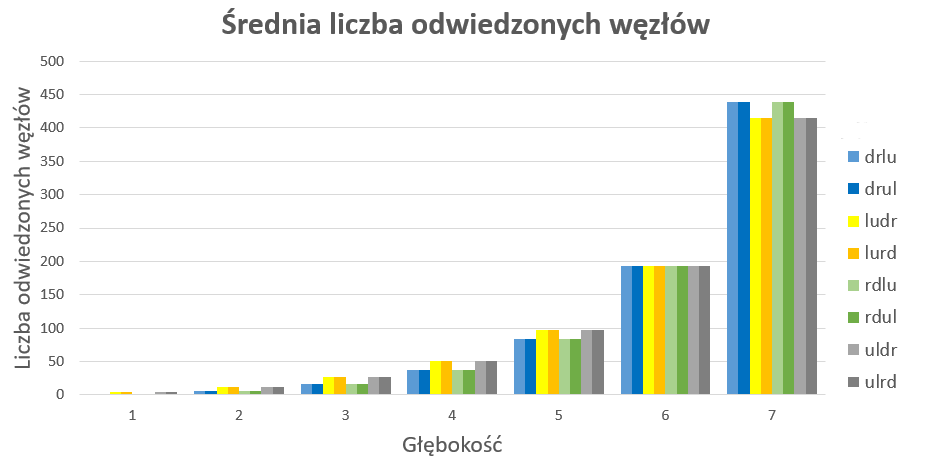
\includegraphics[width=0.83\textwidth]{visitedBFS.png}
    \caption{Średnia ilość odwiedzonych węzłów dla algorytmu BFS}
	\label{visitedBFS}
\end{figure}
\begin{figure}[h!]
    \centering
    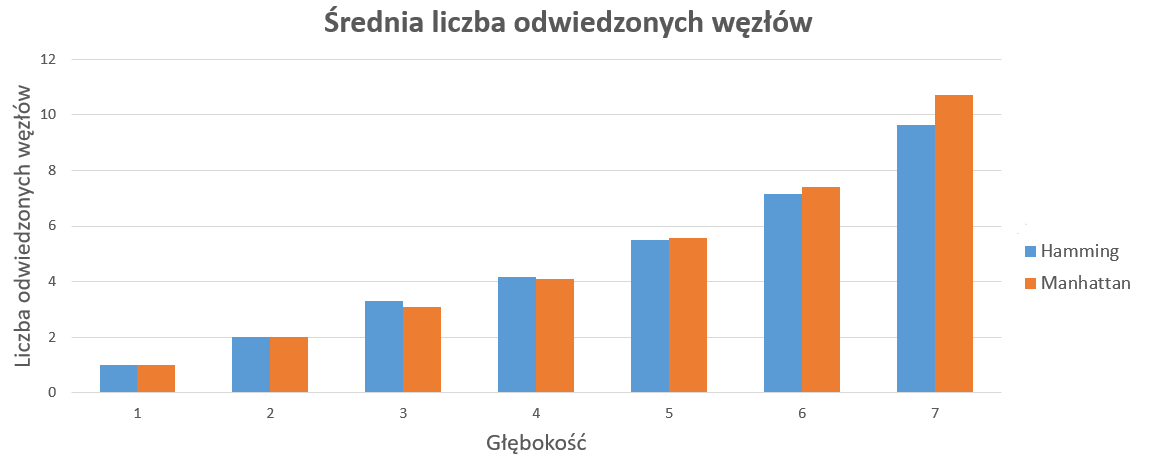
\includegraphics[width=0.83\textwidth]{visitedastar.png}
    \caption{Średnia ilość odwiedzonych węzłów dla algorytmu A*}
	\label{visitedASTR}
\end{figure}

\newpage
\subsection{Długość rozwiązania}
%%%% średnia długość rozwiązania %%%%
\begin{figure}[h!]
    \centering
    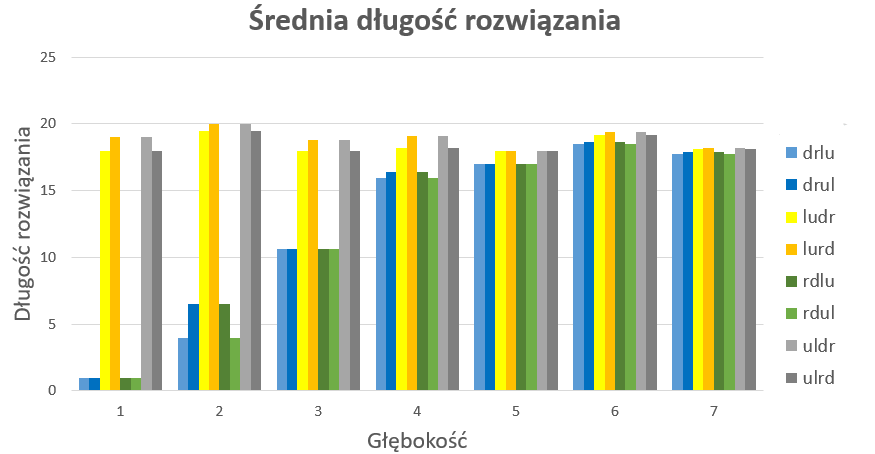
\includegraphics[width=0.83\textwidth]{sredniaDFS.png}
    \caption{Średnia długość rozwiązania dla algorytmu DFS}
	\label{sredniaDFS}
\end{figure}
\begin{figure}[h!]
    \centering
    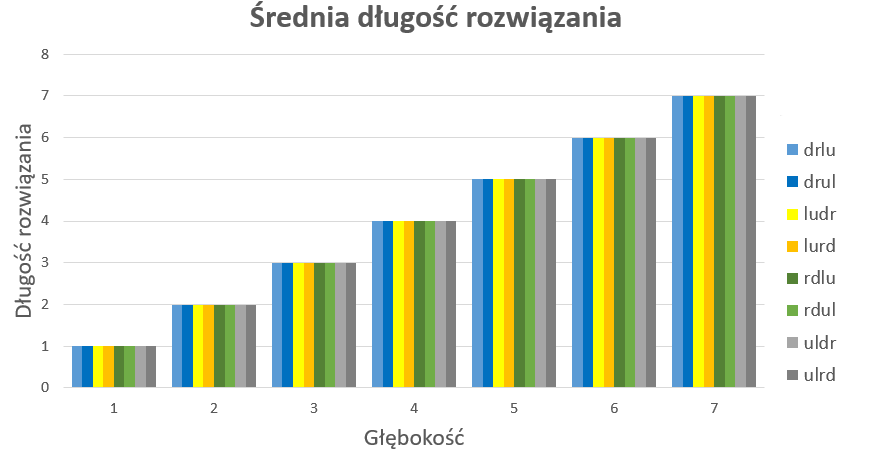
\includegraphics[width=0.83\textwidth]{sredniaBFS.png}
    \caption{Średnia długość rozwiązania dla algorytmu BFS}
	\label{sredniaBFS}
\end{figure}
\begin{figure}[h!]
    \centering
    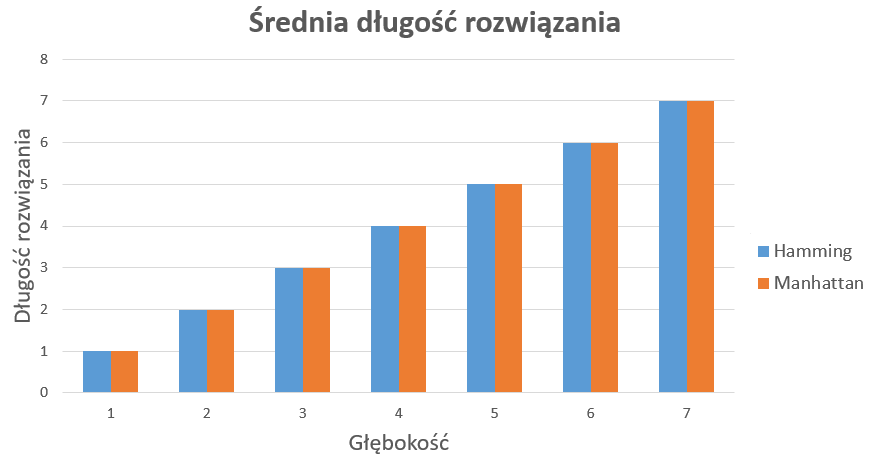
\includegraphics[width=0.83\textwidth]{sredniaastr.png}
    \caption{Średnia długość rozwiązania dla algorytmu A*}
	\label{sredniaASTR}
\end{figure}

\newpage
\subsection{Podsumowanie algorytmów}
%%%% podusmowanie %%%%%%%%%%%%%%%%%%%%%%
\begin{figure}[h!]
    \centering
    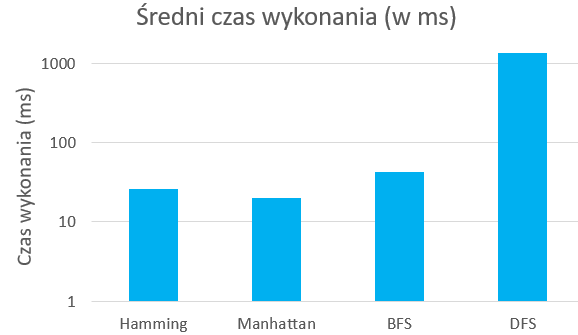
\includegraphics[width=0.75\textwidth]{czasALL.png}
    \caption{Średni czas wykonania - podsumowanie algorytmów}
	\label{czasALL}
\end{figure}
\begin{figure}[h!]
    \centering
    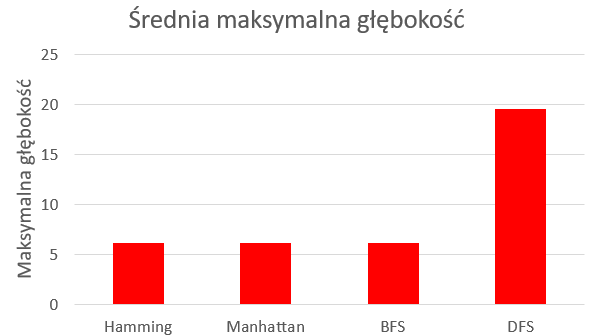
\includegraphics[width=0.75\textwidth]{depthALL.png}
    \caption{Średnia maksymalna głębokość - podsumowanie algorytmów}
	\label{depthALL}
\end{figure}
\begin{figure}[h!]
    \centering
    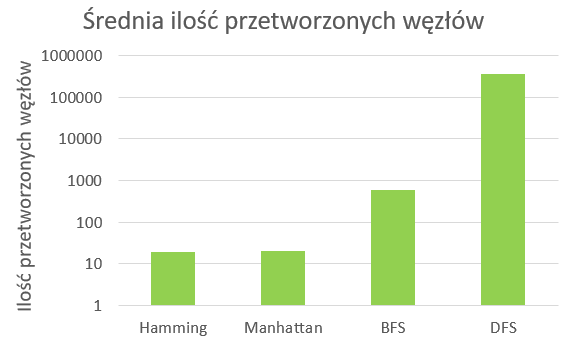
\includegraphics[width=0.75\textwidth]{processedALL.png}
    \caption{Średnia ilość przetworzonych węzłów - podsumowanie algorytmów}
	\label{processedALL}
\end{figure}
\begin{figure}[h!]
    \centering
    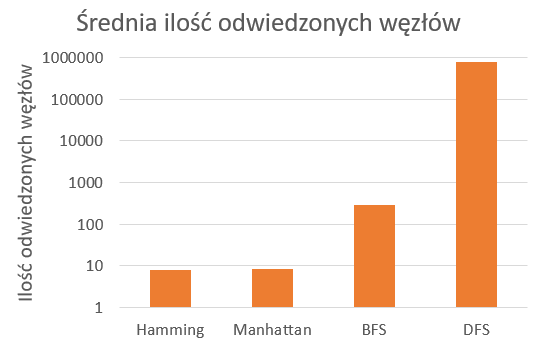
\includegraphics[width=0.75\textwidth]{visitedALL.png}
    \caption{Średnia ilość odwiedzonych węzłów - podsumowanie algorytmów}
	\label{visitedALL}
\end{figure}
\begin{figure}[h!]
    \centering
    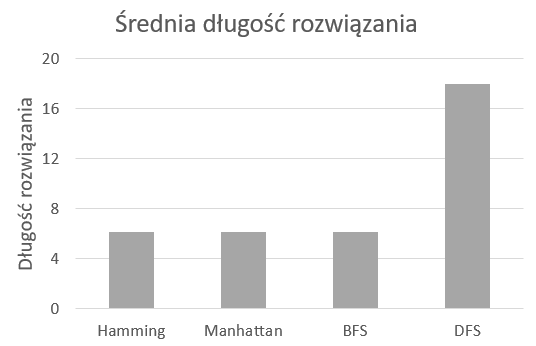
\includegraphics[width=0.75\textwidth]{sredniaALL.png}
    \caption{Średnia długość rozwiązania - podsumowanie algorytmów}
	\label{sredniaALL}
\end{figure}

\newpage
\section{Dyskusja} % 6. Dyskusja  %
\subsection{DFS}
Dla algorytmu DFS wszystkie badane właściwości miały najwyższe wartości, a co za tym idzie - najgorsze. Najszybciej można to porównać z innymi algorytmami na wykresach \ref{czasALL} - \ref{sredniaALL}. Znaleziona średnia długość rozwiązania jest bliska 20, czyli wartości maksymalnej, ustawionej w programie. 

W tym algorytmie bardzo duży wpływ na jego działanie ma priorytet ruchów. W przypadku priorytetów zaczynajacych się kolejnością DR lub RD długość rozwiązania różni się dla głębokości mniejszej od 5. Również można to zauważyć na wykresie średniej liczby przetworzonych i odwiedzonych węzłów (rysunki \ref{processedDFS} oraz \ref{visitedDFS}), jak i również średniej maksymalnej głębokości (\ref{maxdepthDFS}). 
\subsection{BFS}
Ta strategia, w porównaniu do strategii DFS ma znacznie mniejsze wartości, lecz niektóre wartości ma nieco większe niż w przypadku algorytmu A*. Możemy zauważyć, że na wykresie (\ref{sredniaBFS}) długość rozwiązania jest zawsze równa głębokości, więc możemy mieć pewność, że zawsze zostanie znalezione rozwiązanie najkrótsze i najbardziej optymalne. 

Spoglądając na wykresy średniej liczby przetworzonych i odwiedzonych węzłów (rysunki \ref{processedBFS} i \ref{visitedBFS}) można zauważyć, że w przypadku coraz większej głębokości liczba odwiedzonych węzłów znacznie rośnie. Można więc wywnioskować, że jeżeli ta głębokość byłaby jeszcze większa, również czas przetwarzania drastycznie wzrośnie.
\subsection{A*}
W przypadku strategii A* obydwie zastosowane heurystyki dają bardzo podobne i najlepsze wyniki. Średnia długość rozwiązania, ilość przetworzonych czy odwiedzonych węzłów są niemal identyczne, tak samo jak średni czas wykonania (rysunki \ref{czasASTR}, \ref{processedASTR} i \ref{visitedASTR}). Możemy więc śmiało powiedzieć, że ten algorytm jest najlepszy do rozwiązania \textsl{piętnastki}.

\newpage
\section{Wnioski} % 7. Wnioski  %
\begin{itemize}
\item W każdym względzie algorytm DFS jest najgorszy, więc nie powinno się go stosować do rozwiązywania \textsl{piętnastki}.
\item Algorytmy A* niezależnie od wybranej heurystyki są bardzo do siebie podobne i najbardziej optymalne, jednak nie można porównywać ich ze sobą - są do siebie zbyt podobne.
\item Czas przetwarzania algorytmów BFS i DFS zależy w dużej mierze od liczby stanów, dlatego im większa ilość ruchów do wykonania, tym gorzej się sprawują. 
\item Dużą różnicę można zauważyć w stanach odwiedzonych i przetworzonych w algorytmach DFS i BFS, natomiast bliską 0 dla heurystyk Hamminga i Manhattan.
\item Do programu rozwiązującego \textsl{Piętnastkę} najlepszym wyborem będzie strategia A*.
\end{itemize}

\begin{thebibliography}{0}
  	
	\bibitem{pierwszymath} \textsl{http://www.math.ubc.ca/~cass/courses/m308-02b/projects/grant/fifteen.html} [dostęp 17.03.2020]
	\bibitem{wikiDFS} \textsl{https://pl.wikipedia.org/wiki/Przeszukiwanie\_w\_głąb} [dostęp 17.03.2020]
	\bibitem{wikiBFS} \textsl{https://pl.wikipedia.org/wiki/Przeszukiwanie\_wszerz} [dostęp 17.03.2020]
	\bibitem{astr}		\textsl{https://en.wikipedia.org/wiki/A*\_search\_algorithm} [dostęp 17.03.2020]
\end{thebibliography}


\end{document}
